\chapter{Entwurf}
\label{chap:Entwurf}

\section{Anforderungen}
Eine Teilmenge der Anforderungen der domänenspezifischen Sprache wurde bereits in Kapitel \ref{sec:Motivation} in Form von User-Stories aufgeführt. Im Folgenden werden die Anforderungen in einer allgemeineren und umfassenderen Form wiedergegeben. Die zentrale Aussage die den Anforderungen zu Grunde liegt, ist die zusammenfassende Formulierung des zu lösenden Problems: ``Benutzer von MyContactCenter brauchen eine Möglichkeit, das Routing von Konversationsanfragen für eine automatische Kontaktverteilung frei programmieren zu können''. Die Umsetzung dieser Vision ist das langfristige Ziel, sprengt allerdings den Rahmen einer Masterarbeit und damit den der vorliegenden Ausarbeitung. Zwar wurde beim Entwurf Acht darauf gegeben, allen Arten von Konversationsanfragen gerecht zu werden. Für die vorliegende Implementierung beschränkt sich die Ausarbeitung aber lediglich auf das Routing von eingehenden Telefonanrufen. Die relevante Aufgabe lautet also: ``Benutzer von MyContactCenter brauchen eine Möglichkeit, das Routing eingehender Telefonanrufe für eine automatische Kontaktverteilung frei programmieren zu können''.
\newline
Aus dieser Aufgabe ergeben sich folgende Anforderungen für die DSL:
\begin{itemize}
\item Die DSL muss eine Sammlung an Instruktionen bereit stellen, welche mit einem eingehenden Anruf interagieren
\item Instruktionen der DSL müssen sich in einer Reihenfolge arrangieren lassen, welche den zeitlichen Ablauf eines Anrufroutings spezifiziert. Ein solcher Ablauf muss Verzweigungen und Schleifen zulassen.
\item Die Sammlung an Instruktionen müssen folgende Interaktionen mit einem eingehenden Anruf möglich machen:
	\begin{itemize}
	\item Entgegennehmen eines Anrufs
	\item Abspielen von Audiodateien 
	\item Abrufen von Eingaben des Anrufers über Mehrfrequenzwahlverfahren
	\item Ausführen von Benutzerscripten. Bei Bedarf soll ein Benutzer über die Programmiersprache C\# eigene Scripte programmieren können, welche dann im Routing ausgeführt werden.
	\item Einordnen von Anrufen in die Kategorien ``Sprache'' und ``Wissensbereich''. Die Einordnung eines Anrufes in diese Kategorien bestimmt, welche Agenten den Anruf entgegen nehmen können.
	\item Terminieren eines Anrufs
	\item Zustellung eines Anrufs an einen Agenten
	\end{itemize}
\item Ein Ablauf von Instruktionen muss mittels einer grafischen Benutzeroberfläche arrangierbar sein.
\item Ein Ablauf von Instruktionen muss in ausführbaren Code transformierbar sein.
\item Der Ersteller eines Ablaufs von Instruktionen soll durch eine hohe Benutzerfreundlichkeit unterstützt und davor bewahrt werden, unnötige Fehler zu machen.  
\end{itemize}
Die obenstehende Liste stellt die Mindestanforderungen dar, die erfüllt sein müssen, damit ein Benutzer über die gewünschten Konfigurationsmöglichkeiten für eine Automatische Kontaktverteilung verfügt. Der im Folgenden Kapitel beschriebene Entwurf einer domänenspezifischen Sprache ist ein Versuch, ein System zu designen, welches die obenstehenden Anforderungen erfüllt. Zur Umsetzung des Entwurfs wurde ein grafischer Editor und ein Code-Generator umgesetzt, deren Implementierung näher in Kapitel \ref{chap:Implementierung} erläutert wird.

\section{Beschreibung der Sprache}
Die domänenspezifische Sprache ist als grafische Sprache entworfen. Das bedeutet, dass die konkrete Syntax, also das äußere Erscheinungsbild, mit dem der Benutzer interagiert, in Formen und Verbindungen statt in Text ausgedrückt wird. Vergleichbar sind grafische DSLs zum Beispiel mit der Unified Modeling Language (UML), welche allerdings den Anspruch erhebt, eine Universalsprache zu sein [CITATION].
\newline 
In der vorliegend implementierten DSL werden Formen und Linien im zweidimensionalen Raum angeordnet, um das Verhalten des Konversationsroutings zu modellieren. Die Instruktionen der DSL, die mit einer eingehenden Kontaktanfrage interagieren, sind dabei als Rechtecke dargestellt. Es gibt eine Vielzahl von verschiedenen Instruktionen, welche einzeln in folgenden Kapiteln beschrieben werden. Jede Art von  Instruktion ist mit einem Namen eindeutig gekennzeichnet und kann einmal, mehrmals, oder, mit Ausnahme der Start-Instruktion, auch gar nicht in einem Routing auftreten. Das Verhalten von Instruktionen kann parametrisiert sein: Zum Beispiel gibt ein Benutzer bei der Instruktion zum Abspielen einer Audio-Datei die Datei an, die wiedergegeben werden soll. Jedes Instruktions-Rechteck besitzt eine bestimmte Anzahl von Ein- und Ausgängen, symbolisiert durch kleinere Rechtecke, die in der Peripherie des großen Rechtecks eingelassen ist. Die Anzahl an Ein- und Ausgängen eines Rechtecks bestimmen, wie viele ein- beziehungsweise ausgehende Verbindungen für ein Rechteck zugelassen werden und ist für jede Art von Instruktion individuell festgelegt. Eine gerichtete Verbindung in Form eines Pfeils kann zwischen einem Ein- und Ausgang gezogen werden. Dabei geht der Pfeil vom Ausgang aus und zeigt mit der Pfeilspitze auf den Eingang. Während ein Ausgang immer nur eine einzige ausgehende Verbindung hat, kann ein Eingang beliebig viele eingehende Verbindungen akzeptieren. Die Verbindungen zwischen Rechtecken symbolisieren den zeitlichen Ablauf innerhalb des Konversationsroutings: Eine Instruktion A wird dann ausgeführt, wenn eine andere Instruktion B beendet wurde und im Zuge der Ausführung von B ein Ausgang gewählt wurde, der über eine Verbindung zum Eingang von A führt. Welcher Ausgang von B gewählt wird, hängt dabei vom Typ der Instruktion ab. Damit der Benutzer den Kontrollfluss eindeutig modellieren kann, besitzen alle Ausgänge einer Instruktion einen Bezeichner, der andeutet in welchen Situationen dieser Ausgang benutzt wird.  In Abb. \ref{fig:SingleNode} sind die erläuterten Elemente der DSL-Notation mit entsprechender Beschriftung zu sehen.
\newline
Jedes spezifizierte Routing benötigt einen Ausgangspunkt, an dem es seinen Anfang nimmt. Dieser Anfangspunkt ist die Start-Instruktion, welche keinen Eingang und nur einen einzelnen Ausgang hat. Von hier aus wird eine Verbindung zu einer weiteren Instruktion gezogen, welche als erstes im Routing ausgeführt wird. Von hier aus wird nun mit den oben beschriebenen Bausteinen ein Netz von Instruktionen aufgebaut, die den zeitlichen Ablauf eines Konversationsroutings spezifizieren. Ein so spezifiziertes Konversationsrouting ist ein Modell der DSL.
\newline
Ein DSL-Modell kann auch vereinfacht als gerichteter Graph betrachtet werden, in dem die Instruktionen (Rechtecke) die Knoten und die Verbindungen (Pfeile) die Kanten darstellen. Diese Betrachtungsweise ist unter anderem bei der Algorithmik nützlich, welche bei der Implementierung zum Einsatz kam, und ist auch der Grund, warum im Folgenden Instruktionen auch als Knoten bezeichnet werden. 

\begin{figure} %[hbtp]
	\centering
		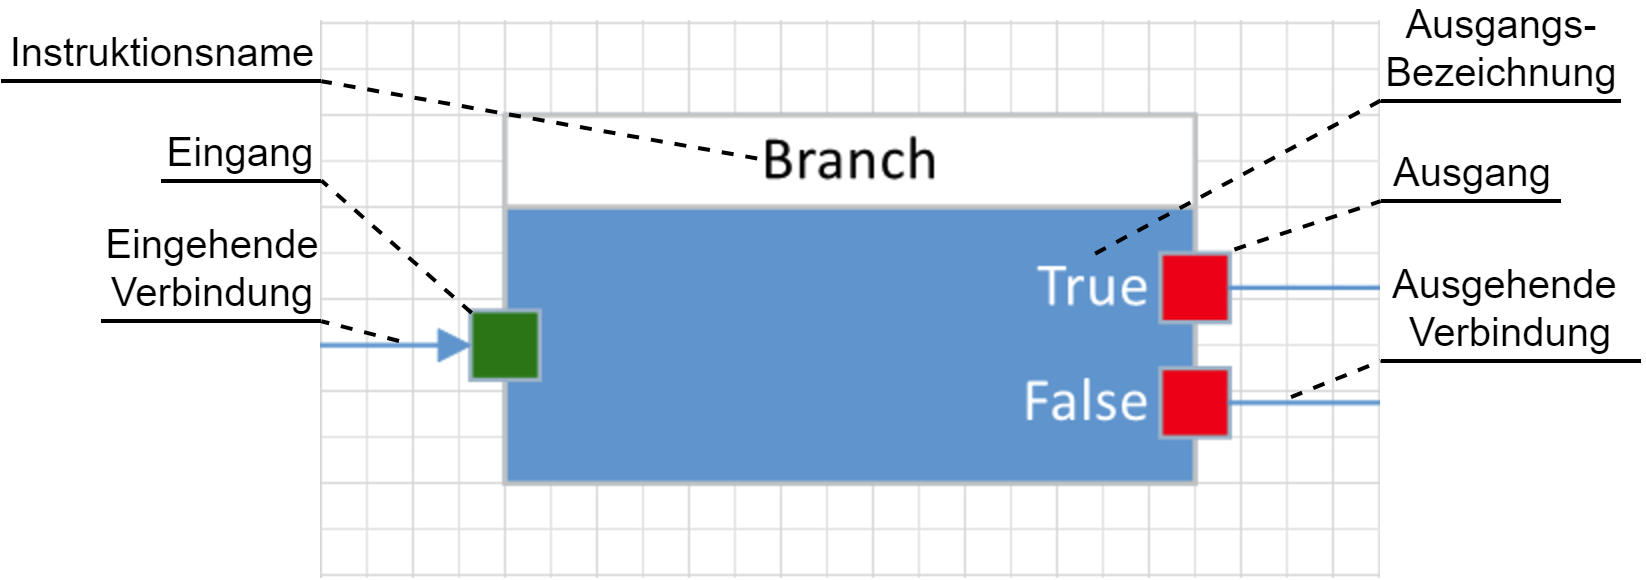
\includegraphics[width=0.8\textwidth]{img/SingleNodeWithAnnotations.png}
	\caption[Beschriftung einer DSL-Instruktion]{Eine einzelne Instruktion wie sie (ohne die Beschriftung) in einem Konversationsrouting dargestellt wird. Abgebildet ist die Branch-Instruktion, welche über einen Eingang und zwei Ausgänge verfügt. Der auszuwertende Ausdruck, welcher den zu nehmenden Ausgang bestimmt, ist nicht in der Instruktion dargestellt, sondern wird auf als Eigenschaft in einem separaten Fenster der Benutzeroberfläche konfiguriert.}
	\label{fig:SingleNode}
\end{figure}

\subsection{Beispiel}
Ein Beispiel soll im Folgenden die Anwendung der domänenspezifischen Sprache näher veranschaulichen. In Abbildung \ref{fig:ExampleRouting} ist ein Konversationsrouting durch ein Modell der DSL spezifiziert. Hier wird für den eingehenden Anruf zu erst eine Fallunterscheidung durchgeführt: Mittels eines C\#-Ausdrucks (dargestellt in der Abbildung durch einen Code-Editor), in dem per System-Aufruf der aktuelle Wochentag ermittelt wird, wird entschieden, ob das Routing an einem Sonntag ausgeführt wird. Ist dies der Fall, wird der Ruf terminiert, da es sich um einen Ruhetag handelt. Andernfalls wird eine DTMF-Abfrage gestartet, bei der dem Anrufer in einer abgespielten Audiodatei ein Menü vorgelesen wird. Braucht der Benutzer zu lange um eine Eingabe zu machen, wird der Timeout-Ausgang gewählt, welcher wieder zurück in die DTMF-Abfrage führt. Bis der Anrufer also eine Eingabe macht oder auflegt, befindet er sich in einer Endlosschleife. Wählt er eine eins, wird er an ein direktes Ziel weitergeleitet. Wählt er dagegen eine 0, wird eine Hintergrundmusik gestartet und er wird in die Warteschlange eingereiht. Nun verbleibt der Anrufer solange in der Warteschleife, bis er auflegt oder ein Agent seinen Anruf entgegennimmt.  

\begin{figure} %[hbtp]
	\centering
		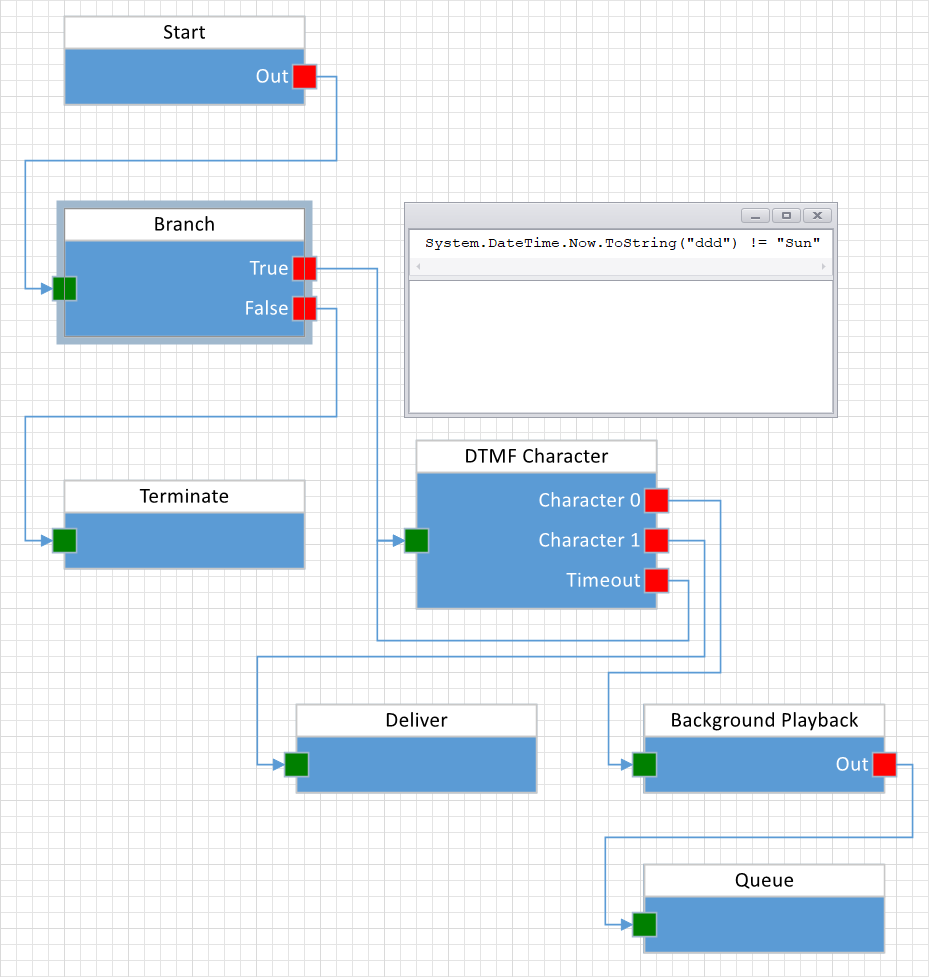
\includegraphics[width=0.79\textwidth]{img/ExampleRoutingRaw.png}
	\caption[Beispiel für ein Konversationsrouting]{Ein beispielhaftes Konversationsrouting}
	\label{fig:ExampleRouting}
\end{figure}

\section{Sprachelemente}
\label{sec:Sprachelemente}
Wie oben beschrieben sind die Hauptelemente der DSL ihre Instruktionen und die Verbindungen zwischen ihnen. Auf welche einzelnen Instruktionen der Benutzer Zugriff hat und wie diese spezifiziert sind, ist im Folgenden beschrieben. 

\subsection{Start}
\begin{labeling}{Anzahl Ausgänge}
\item [Eingang] Nein
\item [Anzahl Ausgänge] 1
\item [Parameter] keine
\item [Beschreibung] Der Start-Knoten ist der Anfangspunkt eines Konversationsroutings. Der Programmfluss erreicht diese Instruktion, wenn ein eingehender Anruf von der Routing Engine angenommen wurde. Der Start-Knoten interagiert selbst nicht mit dem Anruf, sondern führt unmittelbar die im Ablauf vorgesehene folgende Instruktion aus. Die Start-Instruktion muss in jedem DSL-Modell vorhanden sein und ist ein notwendiges Kriterium für eine erfolgreiche Validierung des Modells. 
\end{labeling}

\subsection{Media Playback}
\label{subsec:Media Playback}
\begin{labeling}{Anzahl Ausgänge}
\item [Eingang] Ja
\item [Anzahl Ausgänge] 1
\item [Parameter] Die abzuspielende Audiodatei
\item [Beschreibung] Der Media Playback-Knoten kann vom Benutzer verwendet werden, um Audiodateien abzuspielen. Denkbare Anwendungsfälle sind das Abspielen von Begrüßungsansagen oder Musik-Einspieler. Der Kontrollfluss des Konversationsroutings hält solange bei dieser Instruktion an, wie die Audiodatei dauert und wird erst nach dem Abspielen fortgeführt.  Die abzuspielende Audiodatei muss über die Administration von MyContactCenter vor der Auswahl über einen eigenen Dialog eingespielt werden und wird nach Sprache und Wissensgebiet kategorisiert. Auf diese Weise kann mit dem gleichen Media Playback-Knoten für eine Konversation, die beispielsweise als Englisch kategorisiert ist, eine englische Ansage abgespielt werden während für eine spanische Konversation eine entsprechend spanische Audiodatei abgespielt wird.
\end{labeling}

\subsection{Background Playback}
\begin{labeling}{Anzahl Ausgänge}
\item [Eingang] Ja
\item [Anzahl Ausgänge] 1
\item [Parameter] Die abzuspielende Audiodatei
\item [Beschreibung] Ähnlich wie Instruktion aus Abschnitt \ref{subsec:Media Playback} wird auch bei der Background Playback-Instruktion eine Audiodatei abgespielt. Im Gegensatz zu Media Playback blockiert Background Playback jedoch nicht: Das Konversationsrouting wird mit der nächsten Instruktion fortgeführt. Die abgespielte Audiodatei wird in einer Schleife und im Falle einer weiteren Audiowiedergabe mit geringerer Lautstärke abgespielt. Wird der Ruf an einen Agenten zugestellt wird jegliche Background Playback-Wiedergabe beendet. Background Playback ist vor allem dafür vorgesehen, Hintergrundmusik und ähnliches abzuspielen.
\end{labeling}

\subsection{DTMF Character}
\begin{labeling}{Anzahl Ausgänge}
\item [Eingang] Ja
\item [Anzahl Ausgänge] 13
\item [Parameter] \begin{itemize} \item Eine abzuspielende Audiodatei  \item Dauer des Eingabezeitfensters in Millisekunden \end{itemize}
\item [Beschreibung] Das Mehrfrequenzwahlverfahren (engl. Dual-tone multi-frequency signaling, kurz DTMF) ist eine aus der analogen Telefontechnik stammende Technologie zur Abfrage von Benutzereingaben über eine Telefontastatur [CITATION]. Das Verfahren ist in seiner einfachsten Form daher auf die zwölf Symbole einer Telefontastatur beschränkt: Die Zahlen von null bis neun sowie die Raute und der Asterisk. DTMF ist auch im Session Initiation Protocol implementiert und kann in Konversationsroutings mit der DTMF Character-Instruktion benutzt werden. Wenn der Kontrollfluss auf diesen Knoten trifft, wartet das Routing für das per Parameter vorgesehene Zeitfenster ab, bevor die nächste Instruktion ausgeführt wird. Gibt der Anrufer in dieser Zeit eine Eingabe über seine Telefontastatur ein, wird einer von zwölf Ausgängen gewählt, dessen Bezeichner mit der eingegebenen Taste übereinstimmt. Der dreizehnte mit ``Timeout'' bezeichnete Ausgang wird gewählt, wenn die Zeit des Eingabezeitfenster verstrichen ist und der Benutzer in dieser Zeit keine Eingabe getätigt hat. Zusätzlich ist eine Audiodatei spezifizierbar, welche während des Eingabezeitfensters abgespielt wird.  
\end{labeling}

\subsection{Set Skill}
\label{subsec:Set Skill}
\begin{labeling}{Anzahl Ausgänge}
\item [Eingang] Ja
\item [Anzahl Ausgänge] 1
\item [Parameter] Der zu setzende Wissensbereich
\item [Beschreibung] Damit die automatische Kontaktverteilung von MyContactCenter funktioniert, müssen Konversationen in Sprachen (engl. languages) und Wissensbereiche (engl. Skills) eingeteilt (siehe \ref{sec:MyContactCenter} werden. Die Kategorisierung dieser Konversationen sollte auch innerhalb eines Konversationsroutings möglich sein. Dazu dient die Set Skill-Instruktion, welche der Konversation ein dem System bekannten Wissensbereich zuweist. Der Benutzer kann so aus einer Liste der verfügbaren Wissensbereiche einen Bereich wählen, in den die aktuelle Konversation passt.
\end{labeling}

\subsection{Set Language}
\label{subsec:Set Language}
\begin{labeling}{Anzahl Ausgänge}
\item [Eingang] Ja
\item [Anzahl Ausgänge] 1
\item [Parameter] Die zu setzende Sprache
\item [Beschreibung] Verhält sich für Spachen analog zur Instruktion aus \ref{subsec:Set Skill}.
\end{labeling}

\subsection{Branch}
\begin{labeling}{Anzahl Ausgänge}
\item [Eingang] Ja
\item [Anzahl Ausgänge] 2
\item [Parameter] Ein C\#-Ausdruck der bei Auswertung einen booleschen Wert zurückgibt
\item [Beschreibung] Verzweigungen im Konversationsrouting machen es dem Benutzer möglich, komplexere Abläufe durch Fallunterscheidungen zu modellieren und so mehr Anwendungsszenarien für das Konversationsrouting abzubilden. Solche Verzweigungen werden durch die  Branch-Instruktion möglich. Diese besitzt als Parameter einen frei programmierbaren C\#-Ausdruck, welcher als Boolean auswertbar sein muss. Bei Ausführung einer Branch-Instruktion wird der Ausdruck ausgewertet und je nach Ergebnis einer der beiden mit ``True'' und ``false'' bezeichneten  Ausgänge für die folgende Instruktion ausgewählt.
\end{labeling}

\subsection{Script}
\label{subsec:Script}
\begin{labeling}{Anzahl Ausgänge}
\item [Eingang] Ja
\item [Anzahl Ausgänge] Variabel
\item [Parameter] C\#-Quellcode
\item [Beschreibung] Ein Ziel der domänenspezifischen Sprache ist zwar, dem Benutzer das langwierige Programmieren mit einer Universalsprache zu ersparen. Aber auf diese Weise können nicht alle relevanten Anwendungsfälle abgedeckt werden. In den Fällen, in denen die Sammlung an grundlegenden Instruktionen nicht ausreicht, wird es dem Benutzer ermöglicht, mittels der Script-Instruktion eigenen C\#-Code im Zuge eines Konversationsroutings auszuführen. Der Skript-Code wird direkt als Parameter der Instruktion übergeben und unterliegt gewissen Rahmen-Bedingungen. Es wird nur Code zugelassen, der laut den C\#-Vorschriften in einem Methoden-Körper möglich ist. Damit fallen potentiell gefährliche Operationen wie das Definieren von eigenen Typen oder Funktionen weg. Ebenfalls wird vom Benutzer verlangt, am Ende seines Skripts einen String zurückzuliefern. Dieser String muss identisch mit dem Bezeichner eines der Ausgänge der Skript-Instruktion sein, deren Anzahl und Bezeichner durch den Benutzer festgelegt werden. Auf diese Weise hat der Benutzer innerhalb seines C\#-Skripts die Kontrolle darüber, welcher Ausgang und somit welche Instruktion als nächstes im Konversationsrouting ausgeführt werden. Für eine erfolgreiche Validierung eines Modells muss jeglicher vom Benutzer geschriebene Code compilierbar sein.   
\end{labeling}

\subsection{Deliver}
\label{subsec:Deliver}
\begin{labeling}{Anzahl Ausgänge}
\item [Eingang] Ja
\item [Anzahl Ausgänge] Keine
\item [Parameter] Sip-Uri des Zustellungsziels
\item [Beschreibung] Ein möglicher Endpunkt in einem Konversationsrouting ist die Zustellung an einen Sip User Agent, zum Beispiel einen MyCC-Agenten. Dies wird mit dem Deliver-Knoten erreicht, welcher als Parameter einen United Resource Identifier (URI) als String erhält. URIs werden in SIP zur Identifizierung von User Agents benutzt. Der aktuelle Kontrollfluss des Konversationsroutings gibt an dieser Stelle die Kontrolle über die Konversation an den spezifizierten Teilnehmer ab. Daher besitzt die Deliver-Instruktion keinen Ausgang, mit dem man eine unmittelbare Nachfolgeinstruktion angeben könnte.
\end{labeling}

\subsection{Queue}
\label{subsec:Queue}
\begin{labeling}{Anzahl Ausgänge}
\item [Eingang] Ja
\item [Anzahl Ausgänge] Keine
\item [Parameter] Keine
\item [Beschreibung] Neben der direkten Zustellung an einen Agenten kann ein Anruf auch in der Warteschlange platziert werden, welche dann die automatische Verteilung an einen freien Agenten übernimmt. Dies kann über die Queue-Instruktion erreicht werden. Warteschlangen sind nach Sprache und Wissensbereich kategorisiert und beim Ausführen der Queue-Anweisung wird der eingehende Anruf entsprechend der aktuell eingestellten Sprache und des aktuellen Wissensbereich (siehe Instruktionen \ref{subsec:Set Language} und \ref{subsec:Set Skill}) in eine passende Warteschlange einsortiert. Ist ein Agent bereit den Anruf anzunehmen, wird der Anruf zu diesem Agenten durchgestellt.
\end{labeling}

\subsection{Terminate}
\begin{labeling}{Anzahl Ausgänge}
\item [Eingang] Ja
\item [Anzahl Ausgänge] Keine
\item [Parameter] Grund der Terminierung
\item [Beschreibung] Die Terminate-Instruktion ermöglicht das kontrollierte Beenden des Anrufs durch die Routing Engine. Ähnlich wie die Deliver-Instruktion aus Abschnitt \ref{subsec:Deliver} ist auch die Terminate-Instruktion ein Konversationsroutingendpunkt und besitzt daher keine Ausgänge. Als Parameter nimmt Terminate einen Grund für das Beenden des Rufs entgegen. Der Grund kann aus einer Aufzählung von vordefinierten Anlässen ausgewählt werden.
\end{labeling}

\subsection{Variablen}
\label{subsec:Variablen}
Variablen unterstützen den Benutzer beim Schreiben von eigenem C\#-Code, wie zum Beispiel in Script- oder Branch-Knoten. Variablen können vom Benutzer deklariert werden und sind nicht für eine einzelne Instruktion angelegt, sondern auf Ebene des Konversationsroutings definiert. Sie erscheinen nicht als Rechteck in der Notation wie andere Instruktionen, sind über Dialoge in der grafischen Benutzeroberfläche konfigurierbar. Eine deklarierte Variable kann überall dort im Routing verwendet werden, wo der Benutzer eigenen C\#-Code schreibt. Zur Auswahl für den Variablentyp stehen die primitiven Datentypen int, float, double, bool, string und zusätzlich zur Abbildung von Daten und Zeitpunkten der Typ DateTime aus dem Standard C\#-Namespace System zur Verfügung. Zusätzlich zum Typ muss der Benutzer einen Bezeichner angeben, unter dem die Variable im Konversationsrouting referenziert werden kann. Der Wert einer Variable kann mit der Set Variable-Instruktion gesetzt werden, die in Abschnitt \ref{subsec:Set Variables} erläutert wird. 

\subsection{Funktionen}
Zusätzlich zu Variablen kann der Benutzer eigene Funktionen deklarieren, welche ebenfalls in C\# definiert werden. Ähnlich wie Variablen sind Funktionsdeklarationen keine Instruktion die in der Notation als Rechteck symbolisiert sind, sondern Eigenschaften des Routings. Sie werden daher auch über gesonderte Dialoge der grafischen Benutzeroberfläche angelegt. Für eine Funktionsdeklaration gibt der Benutzer den Bezeichner, eine Liste von Parametern mit Typ und Bezeichner, den Rückgabetyp und den Funktionskörper an. Für alle Typen steht die gleiche Auswahl, die auch bei Variablen angeboten wird, zur Verfügung. Beim Rückgabetyp kann der Benutzer zusätzlich void angeben, um eine Funktion ohne Rückgabe zu definieren. Ist eine Funktion deklariert, kann sie im gesamten Konfigurationsrouting dort aufgerufen werden, wo der Benutzer eigenen C\#-Code angibt.  

\subsection{Set Variables}
\label{subsec:Set Variables}
\begin{labeling}{Anzahl Ausgänge}
\item [Eingang] Ja
\item [Anzahl Ausgänge] 1
\item [Parameter] Eine Sammlung an Variablenzuweisungen
\item [Beschreibung] Wie in \ref{subsec:Variablen} beschrieben werden Variablen-Deklarationen auf Ebene des Konversationsroutings vollzogen und treten nicht als konkrete Instruktion in der grafischen Notation in Erscheinung. Wert-Zuweisungen werden jedoch mittels der Set Variables-Instruktion umgesetzt. Hier kann der Benutzer eine Liste von Zuweisungen hinterlegen. Jede Zuweisung enthält eine Variable aus der Liste der Deklarationen und einen frei programmierbaren C\#-Ausdruck. Führt der Programmfluss die Set Variables-Instruktion aus, werden die Wertzuweisungen ausgeführt.
\end{labeling}

\subsection{Vordefinierte Variablen}
Neben den selbst angelegten Variablen hat der Benutzer in seinen Scripten auch Zugriff auf Variablen die schon von der DSL vorgegeben sind. Dies sind die Variablen Skill und Language, welche jeweils als String verfügbar sind. Diese kann der Benutzer in seinem eigenen Code auslesen, oder setzen. In letzterem Fall wird so die gleiche Funktion erfüllt, die sonst die Instruktionen aus Abschnitt \ref{subsec:Set Skill} und \ref{subsec:Set Language} übernehmen. Setzt der Benutzer die Sprache auf oder den Wissensbereich auf einen Wert, der nicht existiert, wird die Variable nicht verändert. 

\section{Verarbeitungsschritte}
\label{sec:Verarbeitungsschritte}
Zwischen der Modellierung und der letztendlichen Ausführung eines DSL-Modells finden sechs Verarbeitungsschritte statt. Abbildung \ref{fig:Verarbeitungsschritte} veranschaulicht den Vorgang, den ein Konversationsrouting von der Spezifikation bis zur Ausführung durchläuft. Am Anfang steht die Modellierung durch den Benutzer. Hier werden die Instruktionen in einem oben beschriebenen Graphen angeordnet und Verbindungen gezogen, um einen Konversationsroutingablauf zu spezifizieren. Intern und für den Benutzer unsichtbar wird im Editor synchron zu der graphischen Repräsentation eine C\#-Datenstruktur erstellt, welche die abstrakte Syntax als .NET Objekt abbildet (Details zu diesem Vorgang folgen in Kapitel \ref{sec:Editor}). Diese Struktur wird beim Abspeichern des Modells im Protobuf-Format serialisiert und in einer Datenbank abgespeichert. Die serialisierten Daten werden von der Routing Engine abgerufen und deserialisiert. Das Resultat ist die vom Benutzer angelegte C\#-Objekt-Struktur. Die Struktur wird an den Transformator übergeben, welcher die Struktur in konkrete MSIL-Syntax transformiert (wie dies geschieht wird in Kapitel \ref{sec:Transformation} erläutert). Die Routing Engine compiliert die MSIL-Syntax nun im Arbeitsspeicher mit der Hilfe von Roslyn, und erhält eine .NET-MSIL-Assembly. Der Code in dieser Assembly wird anschließend für jeden eingehenden Anruf ausgeführt. 

\begin{figure} %[hbtp]
	\centering
		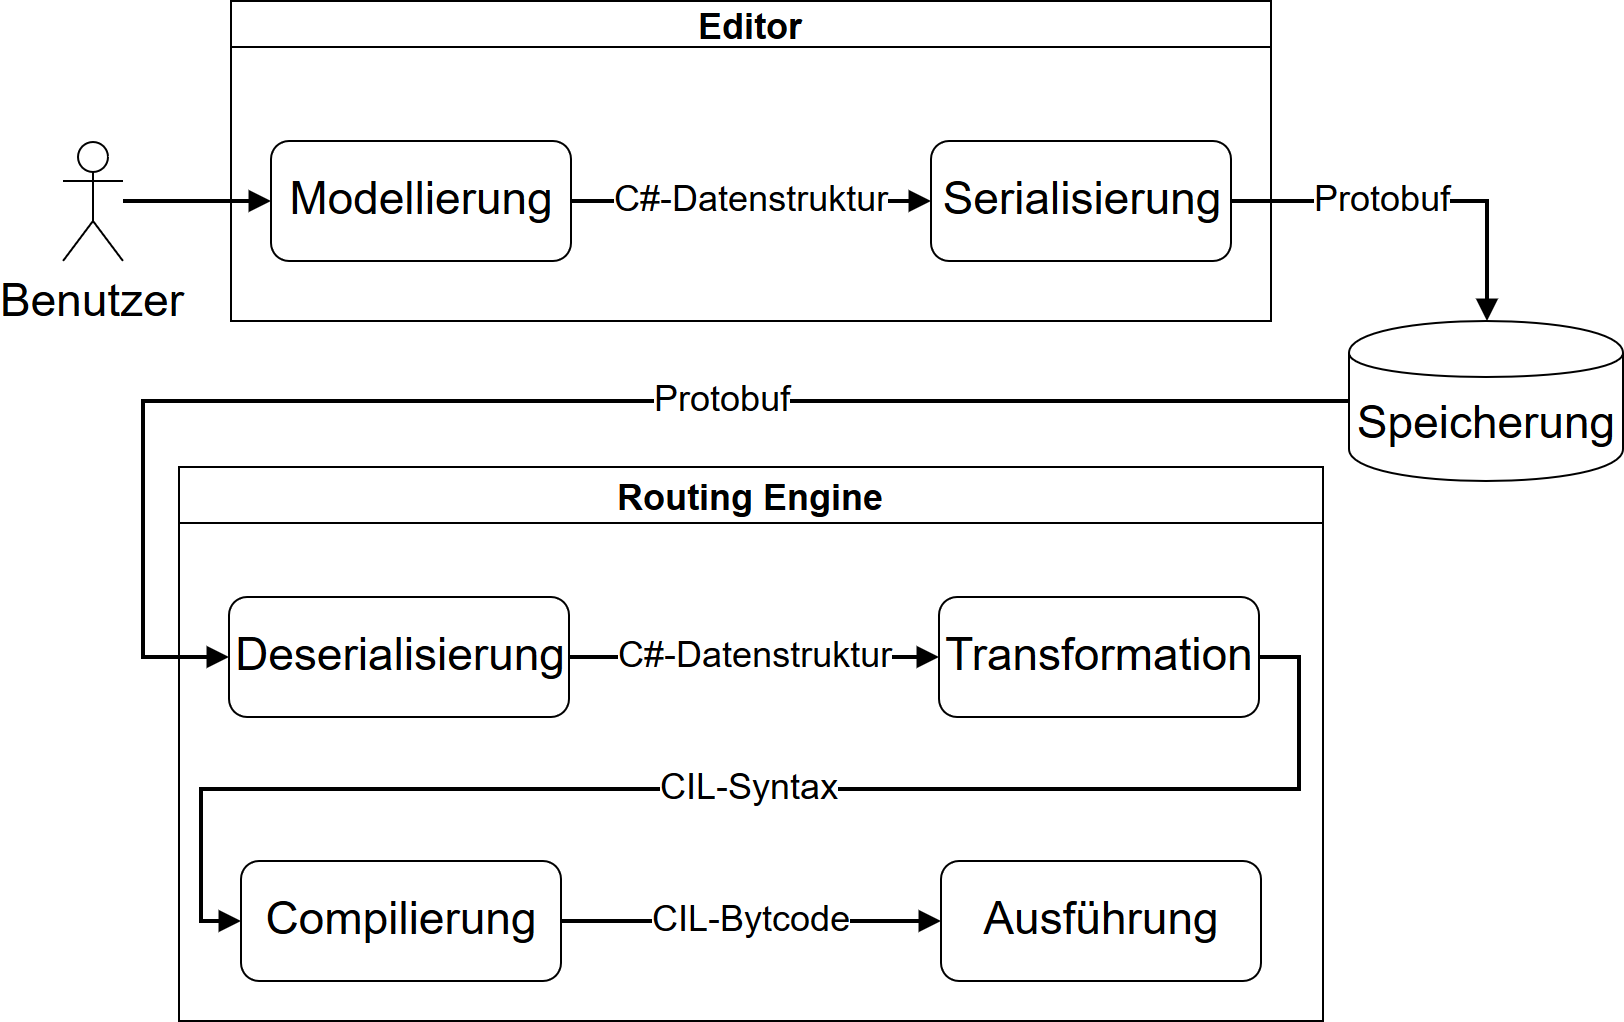
\includegraphics[width=\textwidth]{img/Verarbeitungsschritte.png}
	\caption[Verarbeitungsschritte eines DSL-Modells]{Die Verarbeitungsschritte eines DSL-Modells schematisch dargestellt. Die Schritte sind als abgerundete Rechtecke dargestellt, deren zeitliche Abfolge durch Pfeile gezeigt wird. Die Pfeile sind mit der Eingabe für den jeweils nächsten Verarbeitungsschritt beschriftet. Die Container zeigen an, im Zuge welches Programmcodes die Verarbeitungsschritte ausgeführt werden. Zuerst modelliert der Benutzer einen Ablauf im Editor. Anschließend wird das Modell dort serialisiert und in einer Datenbank abgespeichert. Nach der Deserialisierung in der Routingengine wird das Modell dort transformiert, compiliert und ausgeführt.}
	\label{fig:Verarbeitungsschritte}
\end{figure}